Four categories of systematic uncertainties were considered in the analysis of the data: detector modeling, neutrino interaction modeling, neutrino beam flux predictions, and modeling of secondary hadronic interaction following the primary neutrino interaction.

\subsection{Methodology} 
To determine the impact of an uncertainty, two different formalisms were used. Most uncertainties were evaluated by applying an event-based reweighting factor to the primary simulated neutrino interaction events, and determining the impact on the measured result. For other uncertainties, the generation of re-simulated samples was necessary. 
For the neutrino interaction modeling, beam flux predictions, and secondary hadronic interaction modeling, the systematic uncertainty was determined by applying reweighting factors to simulated events. The use of these weights allows for the complete sampling of the systematic phase space and construction of correlated uncertainties between differential cross-section bins. In the case of the GENIE uncertainty parameters, some parameters have nonlinear dependencies and therefore must be varied simultaneously. Detector modeling uncertainties were estimated by a series of re-simulated samples based on parameters discussed later.
In all cases, covariance matrices are produced capturing the bin-to-bin correlations between uncertainties (a non-negligible effect in these data), which must be used for detailed comparisons with the data.

Uncertainties determined with reweighting factors were evaluated in either a ``multisim" or a ``unisim" approach. The multisim approach varies all parameters from an uncertainty category together and applies the product of all reweighting factors to simulated events as a single weight. On the other hand, the unisim or “1$\sigma$” approach varies each parameter by a shift up or down of one standard deviation individually. The final analysis uses the multisim approach for neutrino interactions, beam flux uncertainties, and secondary hadronic interactions using 1000 sampled universes for each set of uncertainties. 

After determining the systematic uncertainty from each of the four categories, the four uncertainties are then added in quadrature as they are assumed to be fully uncorrelated to each other. The covariance matrices are available in the supplemental material and data release.
The uncertainties as a function of our measured variables are shown in Figs.~\ref{fig:mu_mom_syst} ($p_\mu$), \ref{fig:mu_angle_syst} ($\cos(\theta_\mu$)), \ref{fig:p_mom_syst} ($p_p$), \ref{fig:pangle_syst} ($\cos(\theta_p$)), and \ref{fig:mup_angle_syst} ($\theta_{\mu p}$).
Each figure shows the four main sources of systematic uncertainty, as well as the statistical uncertainty and total uncertainty for each bin.

\subsection{Detector Modeling Uncertainties}
\label{sect:syst_detector}
A variety of effects related to the ability to analyze events in LAr were examined, using actual data whenever possible.
To account for uncertainties in the modeling of ionization yield and drifting of electrons, uncertainties were determined for the following parameters: space charge effect, drift-electron diffusion both transverse and longitudinal, drift-electron lifetime, and drift-electron recombination. 
We vary the magnitude of the space charge effect based upon early measurements of the spatial distortions at the edge of the TPC, extrapolated to the bulk field.
The nominal drift-electron transverse and longitudinal diffusion parameters are set to be the central value of measurements in liquid argon and the variations are based upon the spread of those measurements~\cite{LI2016160}.
The drift-electron lifetime was changed from the nominal value (100~ms) to the lowest measured lifetime of any run period of the detector operations (10~ms) and scaled to the 10\% of the data represented by that low lifetime.  Drift-electron recombination uncertainty was estimated by comparing the nominal simulation which models electron-ion recombination using the modified box model with parameters fit to ArgoNeuT data~\cite{Acciarri_2013} to the variation which substitutes the Birks model~\cite{birks_model} with parameters tuned to ICARUS data~\cite{ICARUS_recomb}.

The shapes of signals on the detector anode wires has uncertainties from dynamically induced charge, intrinsic anode wire and electronics response, and the existence of unresponsive channels. Dynamically induced charge is the creation of electronic signals on anode wires other than the wire closest to the path of drifting electrons, including collection plane wires. In the default simulation this effect is not included, and the variation adds simulation of induced signals on the 10 closest wires. Anode wire response was measured in data~\cite{Adams:2018gbiPROCESS}, and the nominal width is increased based upon the 1$\sigma$ uncertainty of that measurement.  The map of unresponsive channels was used to completely remove any response from those channels which don't respond in data. 
  
To account for uncertainties in the response of the detector to light, uncertainties were determined for light yield, photo-electron noise in PMTs, and light production outside of the TPC. The light yield was varied to cover the differences in scintillation light production in liquid argon based upon modeling different particles types instead of exclusively electrons. The photo-electron noise in the PMTs was varied by $\pm$1$\sigma$ of the measured yield from data. The production of light outside of the TPC may be incorrectly modeled so a sample with light yield outside the TPC increased by 50\% was generated.

The uncertainties from detector modeling are estimated using the unisim method.  For each of the listed detector modeling parameters, the same simulated GENIE v2 neutrino sample of events is reprocessed through GEANT4 with the modified detector parameter. The uncertainty for that parameter is determined by taking the difference in the measured cross section using the nominal measurement or the modified sample and treating this difference as a 1$\sigma$ Gaussian uncertainty for the cross section. For parameters that have both an upward and a downward variation,
we conservatively take the variation that leads to the largest uncertainty and treat this as a 1$\sigma$ uncertainty on the cross-section measurement. The various detector modeling uncertainties are then added in quadrature to determine the total detector uncertainty. 
The largest single uncertainty - leading to an uncertainty of 18\% on the integrated cross section and up to 40\% at $\cos \theta_{\mu}^{\text{reco}} = 0$ - comes from the modeling of dynamically induced charge on the induction wires of the anode. 
These induced signals can interfere with the ``primary'' signal, leading to cancellation of induction plane signals and smearing of collection plane signals, reducing the tracking efficiency in some regions of angular phase space and degrading the charge resolution.
This effect is more successfully modeled in later detector response simulations and will be less significant in future measurements. The detector uncertainty is on average approximately 30\% but can be as high as 50-60\% in some specific regions of phase space.

\subsection{Neutrino Interaction Uncertainties}
\label{sect:syst_genie}

GENIE provides a reweighting framework for the evaluation of the uncertainties from parameters contained in the GENIE models.  The GENIE authors provide estimated uncertainties for various parameters which are mostly determined from fits to external data. For a given parameter $P$, GENIE provides a modified event weight based upon uncertainty $\sigma_P$ that is applied to the sample events and creates a systematically varied distribution. The full list of parameters varied within the GENIE framework can be found in \cite{Andreopoulos:2015wxa}. Beyond the uncertainties on parameters provided in the GENIE model, two additional uncertainties in the neutrino interaction modeling were considered for this measurement. 
We reweight events as a function of true energy transfer and true momentum transfer, according to the ratio of our nominal model (GENIE v2, see Sec.~\ref{sec:evgen}) and the Valencia  model~\cite{Nieves:2004wx,Gran:2013kda}.
This is done separately for CCQE and $2p2h$ 
events, and each uncertainty is added in quadrature to the multisim GENIE uncertainties to obtain the total uncertainty from neutrino interaction modeling.
This sum is labeled as ``Interaction" in Fig.~\ref{fig:mu_mom_syst}-\ref{fig:mup_angle_syst}.
The impact of these uncertainties on the detection efficiency or resolution is very small; the largest impact from these uncertainties is due to changes in background components which we do not constrain.
As the dominant backgrounds are out-of-fiducial-volume and overlaid cosmics, which both scale linearly with the total event rate, the dominant uncertainties are those that change the total rate of predicted neutrino interactions in the MicroBooNE detector.
Parameters that change the shapes of signal or background kinematics, including final state interactions, do not lead to substantial uncertainty on the final measurement.
The neutrino interaction uncertainty is approximately 6\% for most bins of differential cross section with the largest contribution to uncertainty in the lowest bin of muon momentum at 25\%.


\begin{figure}
    \centering
    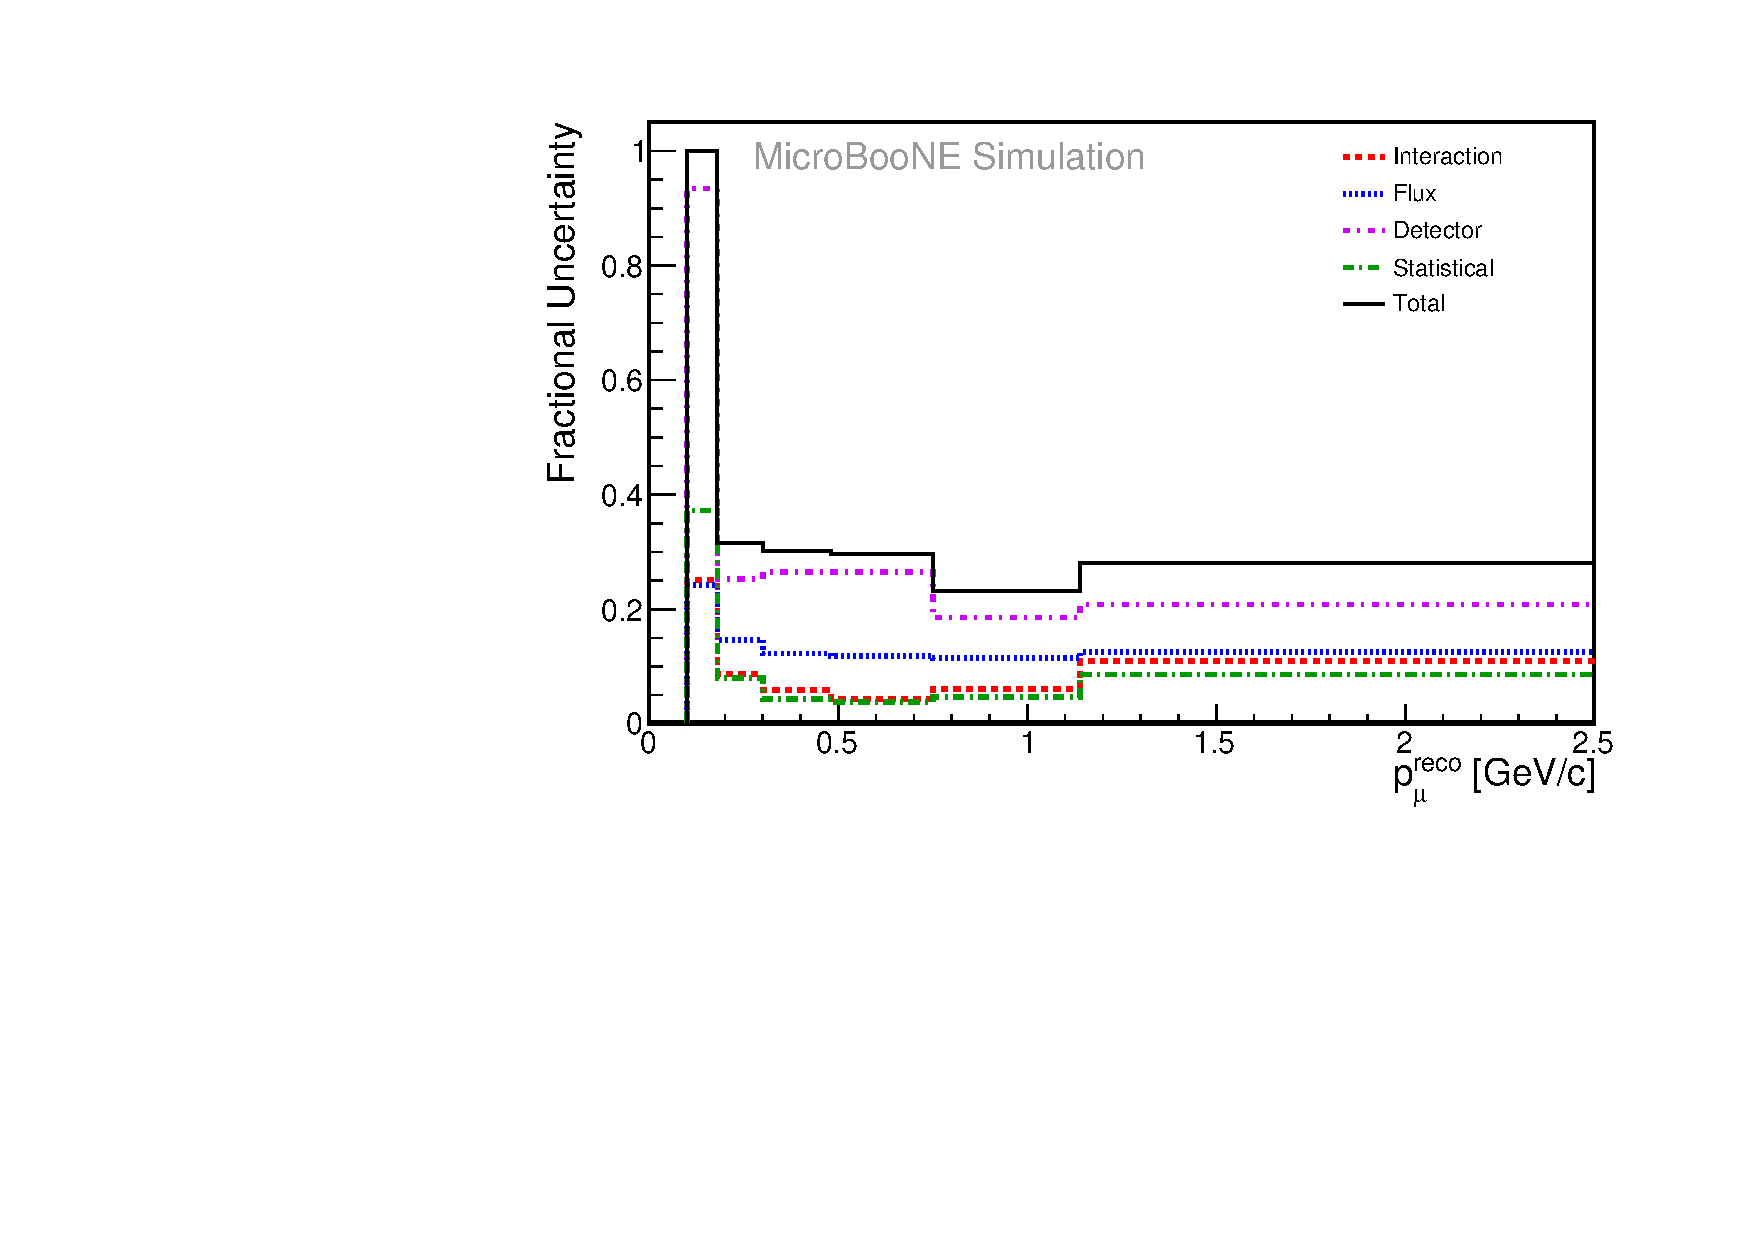
\includegraphics[width=0.45\textwidth]{syst_xsec_may20/Relative_unc_mumom_aug20.pdf}
    \caption{Uncertainties for muon candidate momentum ($p_{\mu}$).}
    \label{fig:mu_mom_syst}
\end{figure}

\begin{figure}
    \centering
    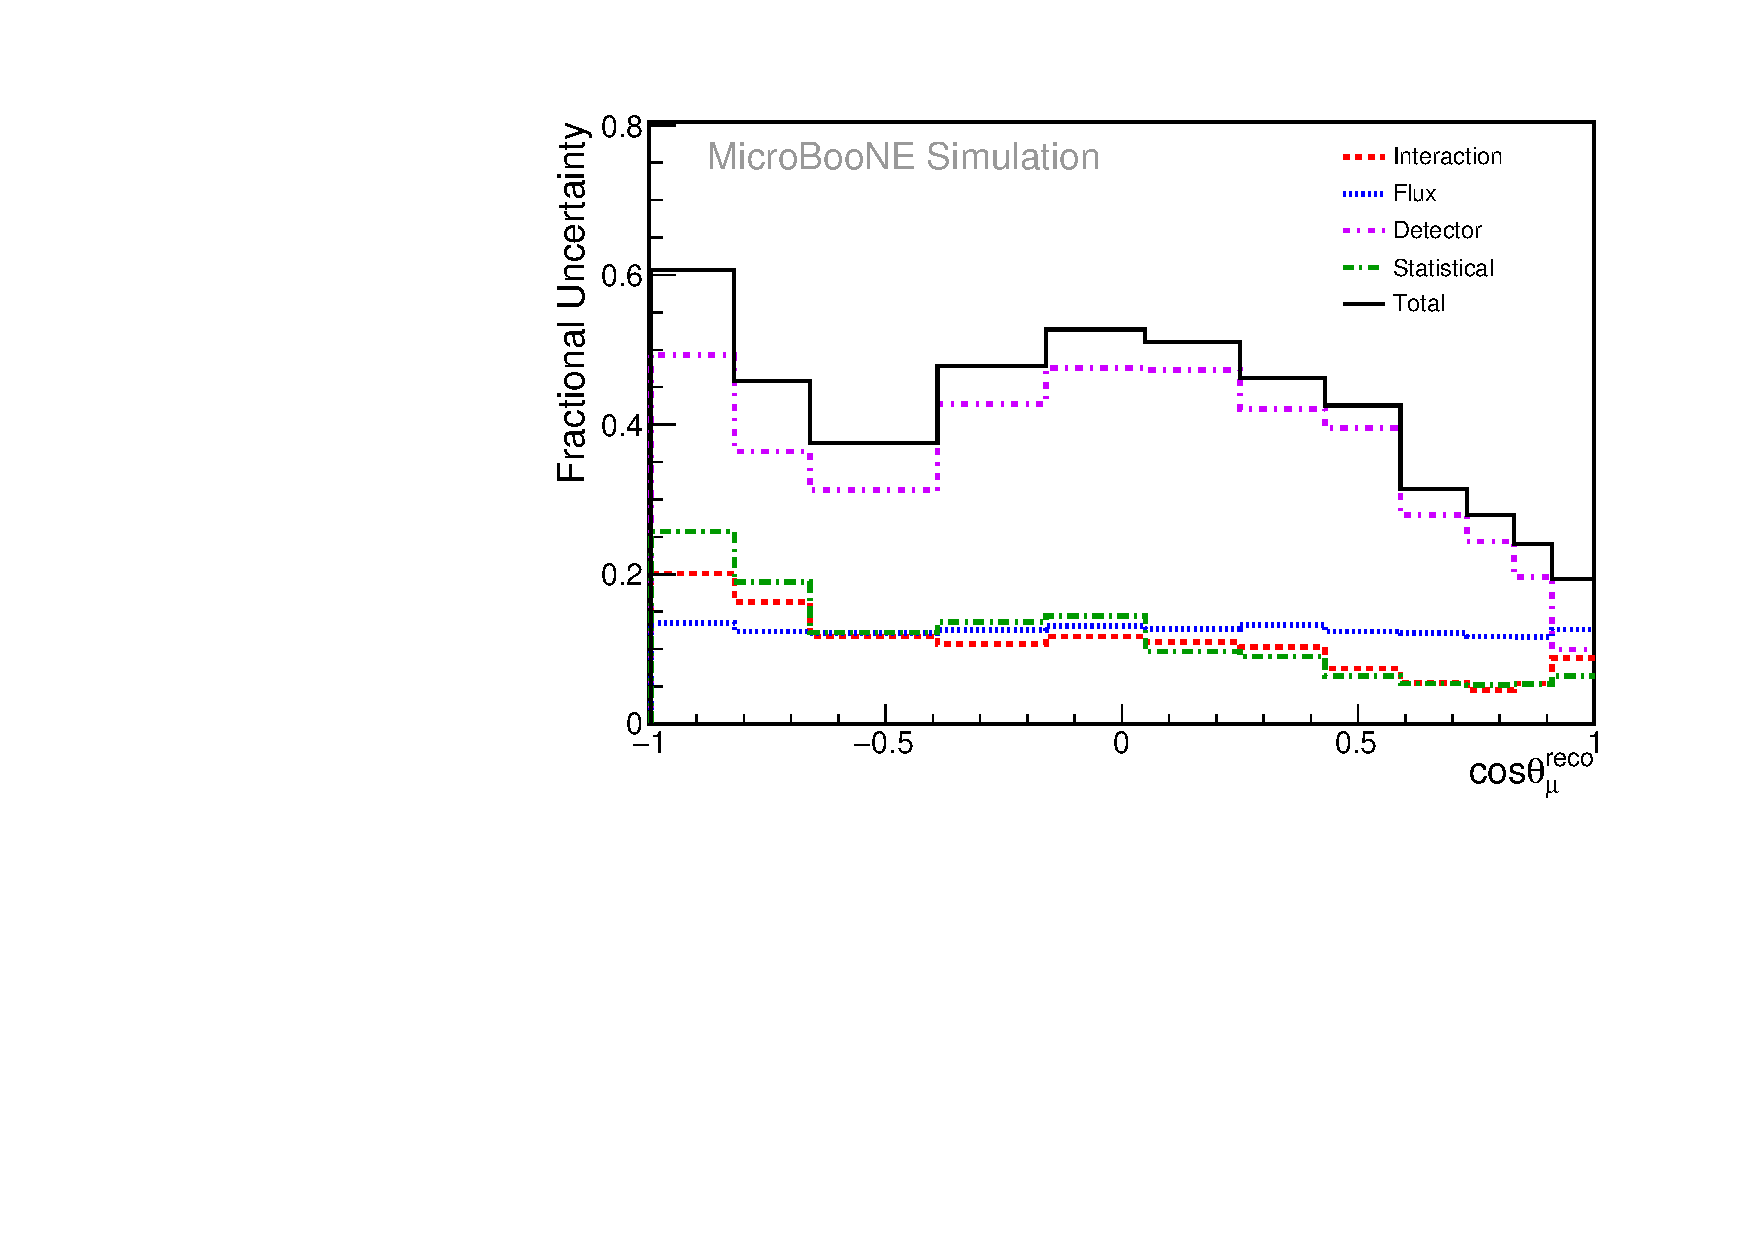
\includegraphics[width=0.45\textwidth]{syst_xsec_may20/Relative_unc_muangle_aug20.pdf}
    \caption{Uncertainties for cosine of the muon polar angle ($\cos \theta_{\mu}$).}
    \label{fig:mu_angle_syst}
\end{figure}

\begin{figure}
    \centering
    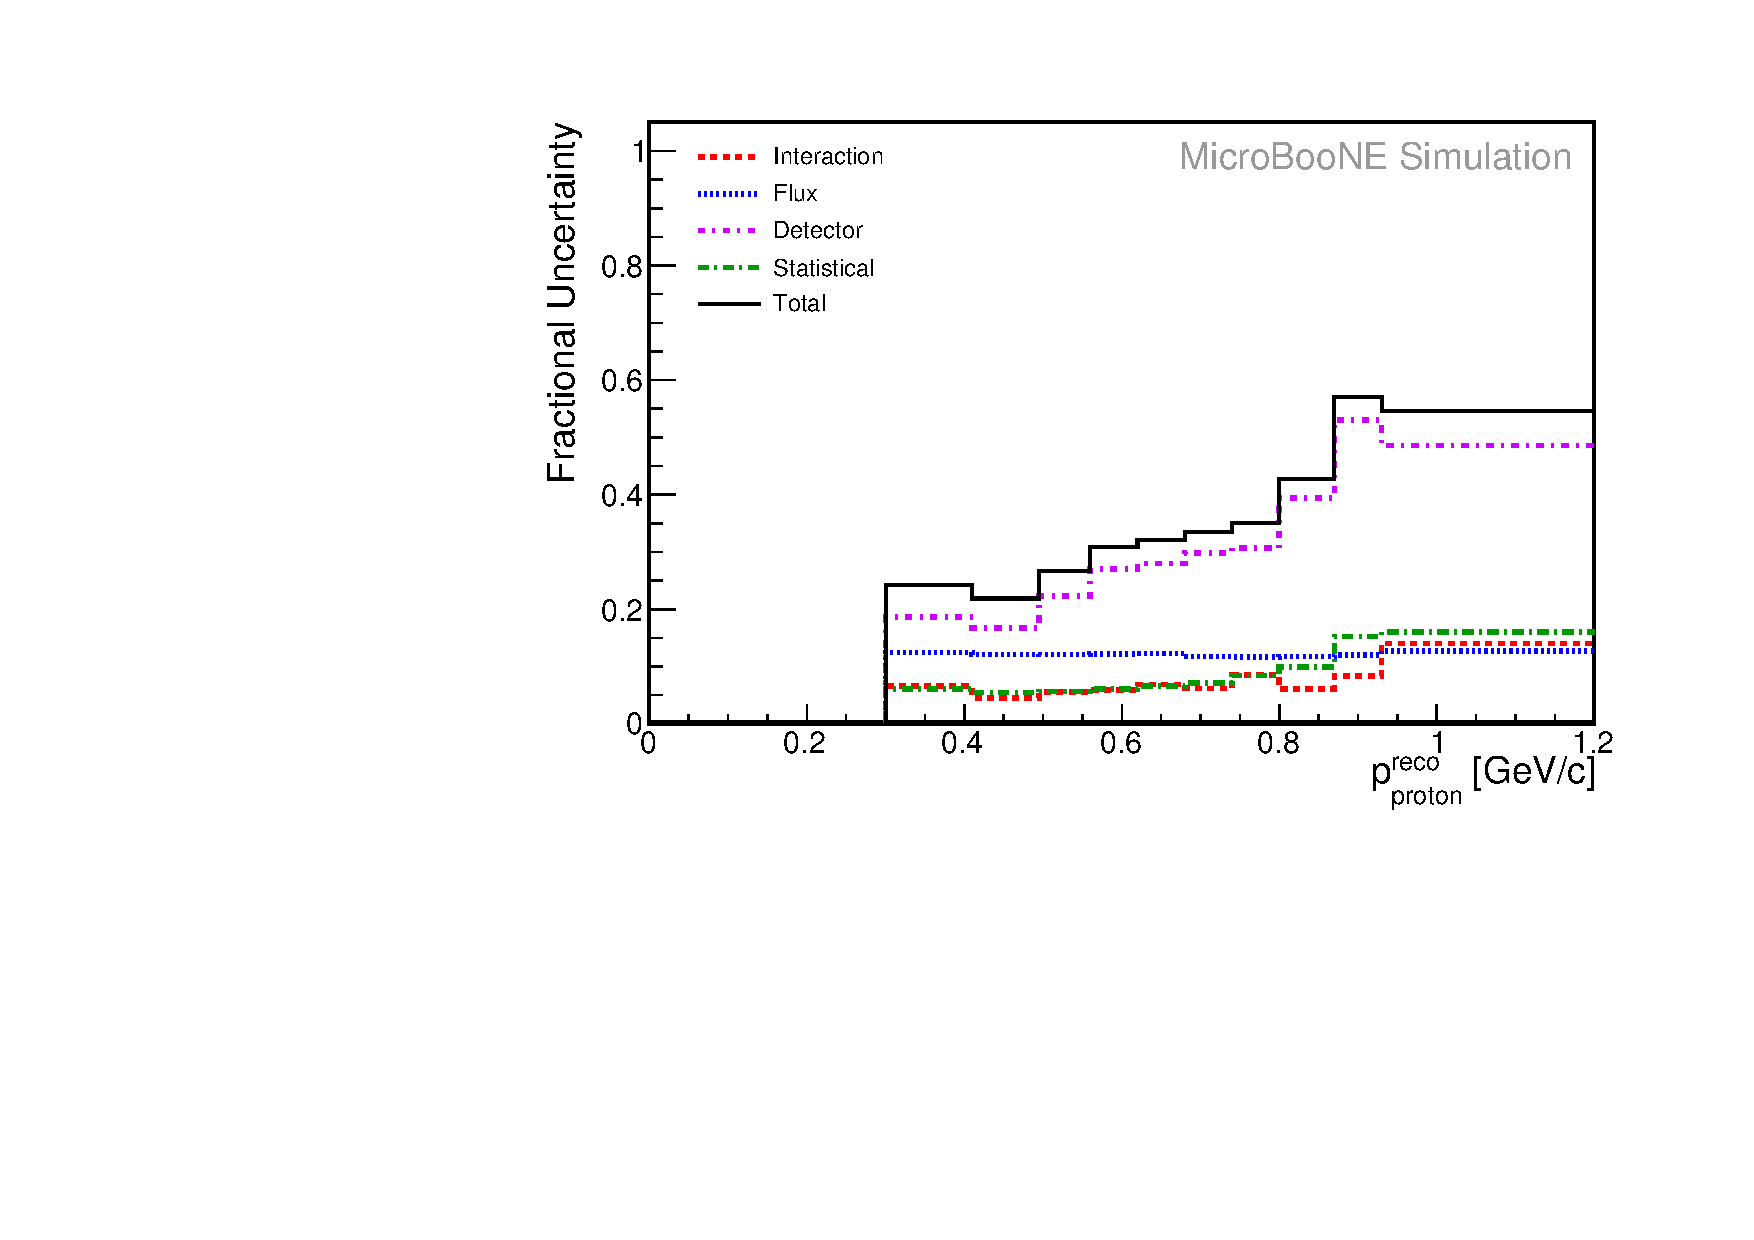
\includegraphics[width=0.45\textwidth]{syst_xsec_may20/Relative_unc_pmom_aug20.pdf}
    \caption{Uncertainties for leading proton candidate momentum ($p_{p}$).}
    \label{fig:p_mom_syst}
\end{figure}

\begin{figure}
    \centering
    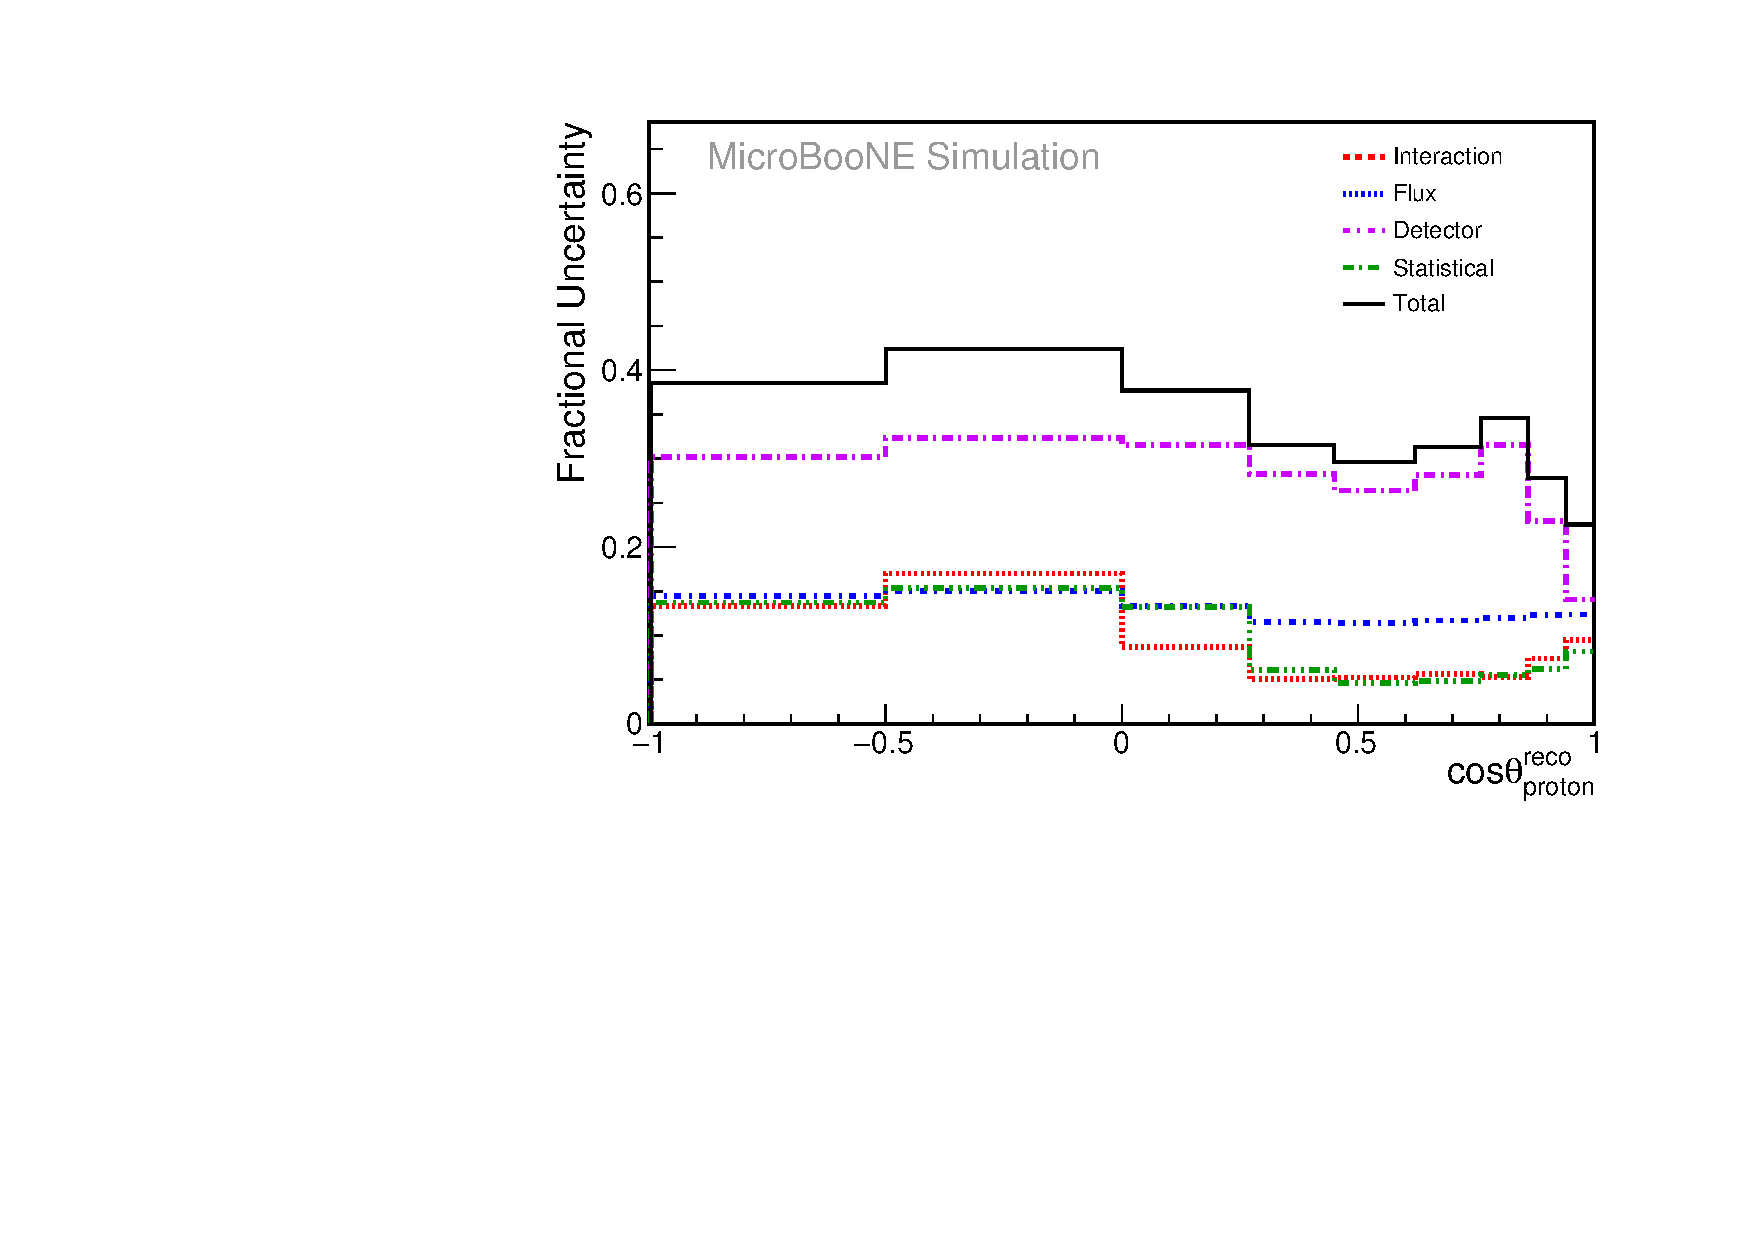
\includegraphics[width=0.45\textwidth]{syst_xsec_may20/Relative_unc_pangle_aug20.pdf}
    \caption{Uncertainties for cosine of the polar angle of the leading proton candidate ($\cos \theta_{p}$).}
    \label{fig:pangle_syst}
\end{figure}

\begin{figure}
    \centering
    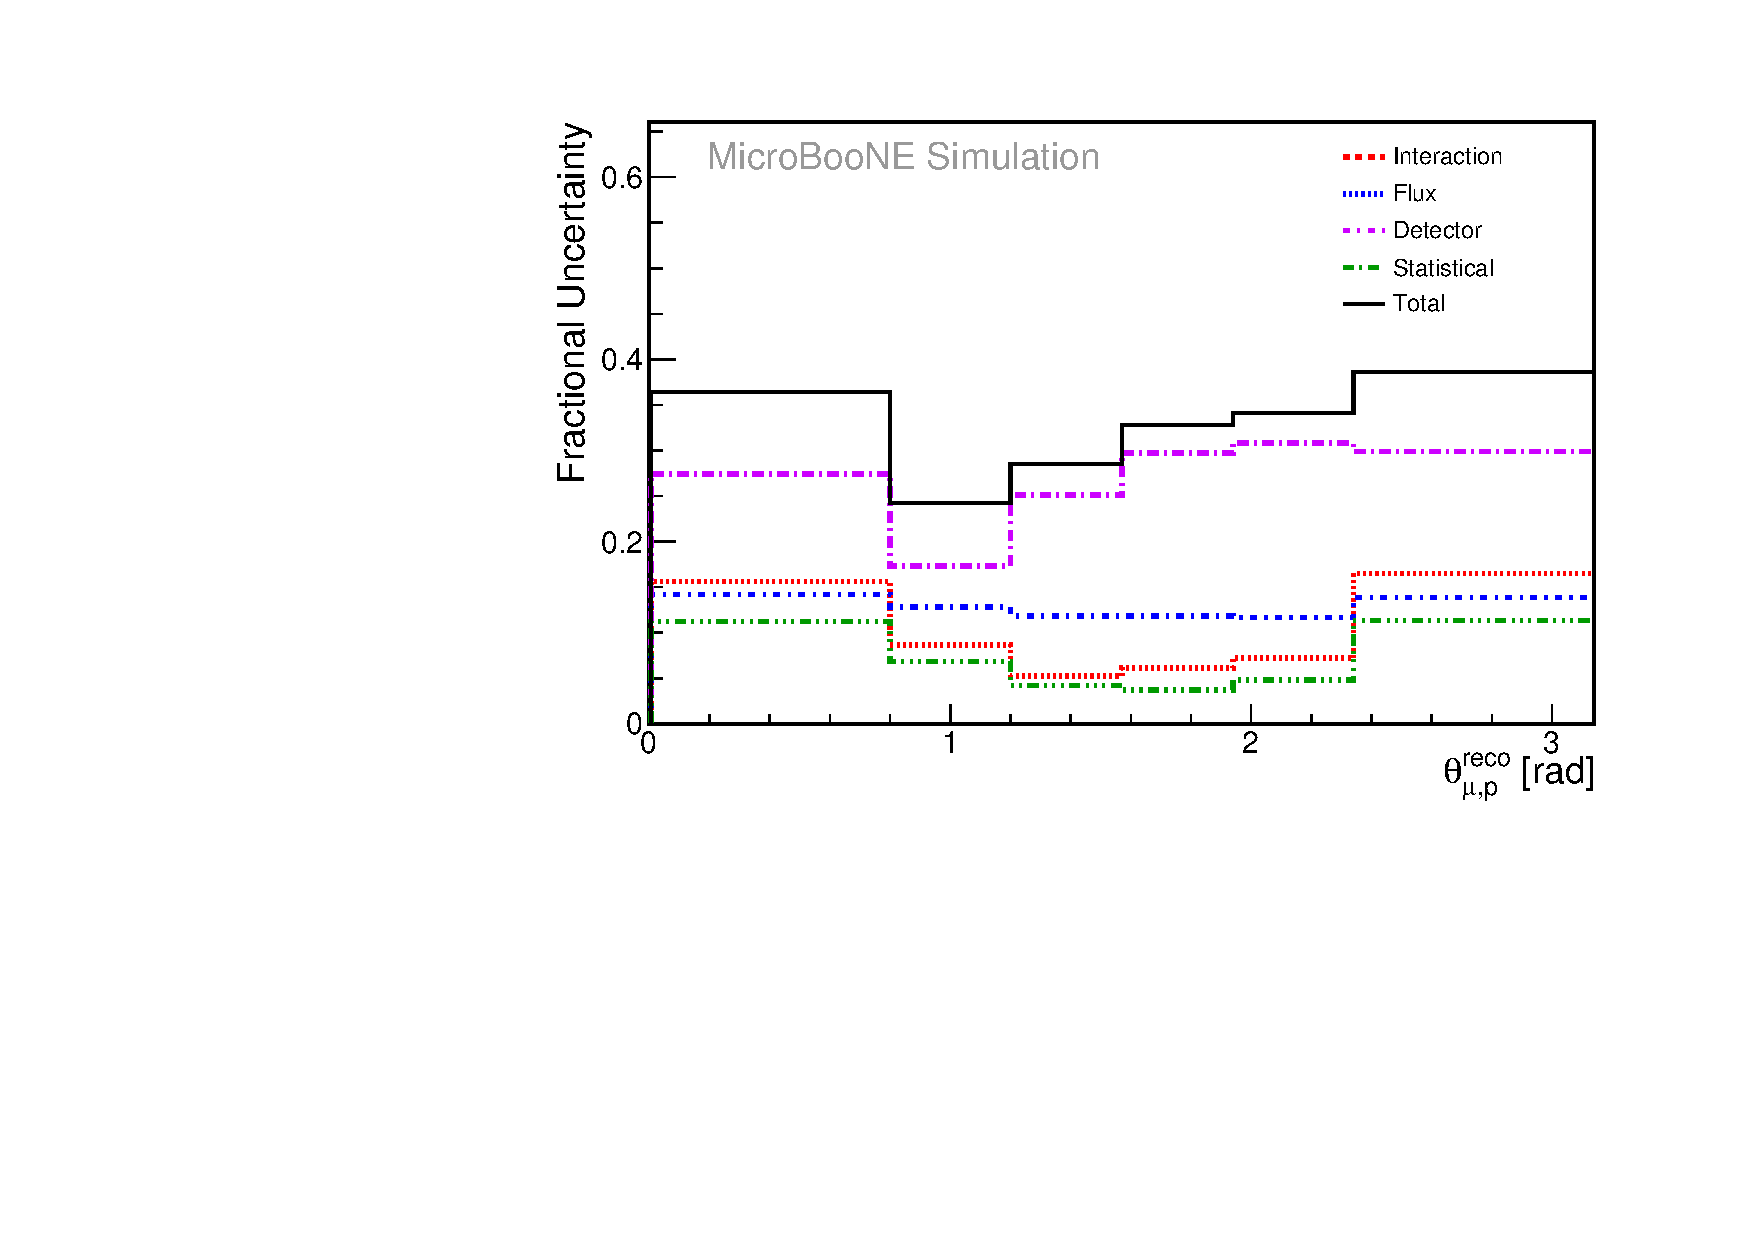
\includegraphics[width=0.45\textwidth]{syst_xsec_may20/Relative_unc_thetamup_aug20.pdf}
    \caption{Uncertainties for the opening angle between muon candidate and leading proton candidate ($\cos \theta_{\mu p}$).}

    \label{fig:mup_angle_syst}
\end{figure}

\subsection{Beam Flux Uncertainties}
\label{sect:syst_beam_flux}
There are two major sources of systematic uncertainty in predicting the neutrino beam flux: hadron production rates and horn focusing effects.
The hadron production rate uncertainties cover the rate of particles produced from protons striking the horn target with variations in $\pi^+$, $\pi^-$, $K^+$, $K^-$, and $K^0$.
These variations are addressed using the multisim approach.
The uncertainty from focusing horn current measurements is estimated using a unisim approach where the beamline is re-simulated with the horn current set at a value 1$\sigma$ away from the nominal.
The multisim hadron production rate uncertainty and the unisim horn current uncertainty are then added in quadrature to give a total beam flux uncertainty. 
The overall uncertainty on the neutrino flux is dominated by an approximately 11\% uncertainty on the absolute normalization, with small uncertainties on the flux shape~\cite{AAAA_2009_MBflux}.
For this reason, the largest impact these uncertainties have on the final cross section measurement is a fully correlated normalization uncertainty of 11\%.
Second order effects from the background subtraction increase this to 15\% in low-purity bins and one bin as high as 25\%.

\subsection{Secondary Hadronic Interaction Modeling}
\label{sect:syst_had_int}
Protons and charged pions can scatter, both elastically and inelastically, in the detector through hadronic interactions with nuclei. These interactions can lead to the production of additional particles or large angle changes in particle trajectories that may lead to reconstruction algorithms failing to form a single, well-reconstructed track.
Interactions such as these can impact the signal efficiency or the background rejection rate, and uncertainties on the rates of these hadronic interactions are propagated to uncertainties on the cross-section measurement. Studies were performed separately for elastic and inelastic interactions, and elastic-scatter uncertainties were found to have negligible impact.

GEANT4 is used to propagate all hadrons through the detector medium based on a semi-classical cascade model~\cite{Wright:2015xia}.  Events with inelastic hadronic interactions are reweighted independently for interactions containing protons, positive pions, and negative pions. For each particle type, the total inelastic cross section is varied around its mean by 30\%, independent of the particle's energy. The pion interaction rate has a negligible impact on the analysis - less than 1\%, while the proton interaction probability does have an impact on the event selection efficiency.
The probability that a proton undergoes an inelastic interaction somewhere along its length increases with trajectory length, so it follows that the impact of proton reinteraction uncertainties is largest at high proton momenta. The uncertainty from proton reinteractions is 8\% at the highest proton energies. 
Events with high proton momemtum tend to have high energy transfer from the lepton, meaning this uncertainty at high proton momentum impacts the measurement of low muon momenta and backwards muon angles.
When this effect is averaged over other variables, the estimated uncertainty from secondary hadronic interaction modeling is 2\%.

In Figs. \ref{fig:mu_mom_syst} - \ref{fig:mup_angle_syst} these uncertainties are added in quadrature to the detector uncertainty.
